\documentclass{article}
\usepackage[T1]{fontenc}
\usepackage[utf8]{inputenc}
\usepackage{lmodern}
\usepackage{amsmath}
\usepackage{sansmath}
\AtBeginDocument{\sansmath}
\renewcommand{\familydefault}{\sfdefault}
\usepackage[paperwidth=19cm,paperheight=14cm,margin=0.4cm]{geometry}
\usepackage{graphicx}
\usepackage{tikz}
\usetikzlibrary{positioning,fit,calc,arrows.meta,backgrounds,decorations.pathreplacing}
\pagestyle{empty}
\setlength{\parindent}{0pt}
\graphicspath{{img/}}

\definecolor{ink}{HTML}{0A0A0A}
\definecolor{muted}{HTML}{6A6A69}
\definecolor{line}{HTML}{BDBDBA}
\definecolor{red}{HTML}{E03A3A}
\definecolor{blue}{HTML}{2E6FE0}
\definecolor{yellow}{HTML}{D9A11A}
\definecolor{green}{HTML}{23A06A}
\definecolor{model}{HTML}{8C8C8A}

\tikzset{
  every picture/.style={font=\sffamily\small, line cap=round, line join=round},
  flecha/.style={-{Stealth[length=2.3mm,width=1.7mm]}, line width=0.7pt, draw=ink},
  grupo/.style={draw=#1, dash pattern=on 3pt off 2pt, line width=0.8pt, rounded corners=2pt, inner sep=6pt},
  titulo/.style={font=\sffamily\small\bfseries, text=#1, anchor=south west, inner sep=1pt},
  foto/.style={inner sep=0pt, outer sep=0pt, draw=ink, line width=0.5pt},
  caja/.style={draw=ink, line width=0.5pt, fill=#1, text=white, font=\sffamily\scriptsize\bfseries,
    text width=3.75cm, minimum height=0.46cm, align=center, inner sep=1.5pt},
  nota/.style={font=\sffamily\scriptsize, text=muted, align=center, inner sep=1pt},
  etapa/.style={font=\sffamily\footnotesize\bfseries, text=ink, align=center, inner sep=1pt},
  paso/.style={draw=ink, line width=0.5pt, fill=#1, text=ink, font=\sffamily\scriptsize, align=center,
    inner sep=3pt, minimum height=0.95cm, text width=2.35cm},
  paso/.default=white,
  grupofondo/.style={draw=#1, line width=0.8pt, fill=#1!6, rounded corners=3pt, inner sep=7pt},
  llave/.style={decorate, decoration={brace, mirror, amplitude=5pt, raise=2pt}, line width=0.7pt, draw=#1},
  llavetexto/.style={font=\sffamily\small\bfseries, text=#1, align=center},
}

\begin{document}
\begin{tikzpicture}

\node[foto] (in) at (0, 1.75) {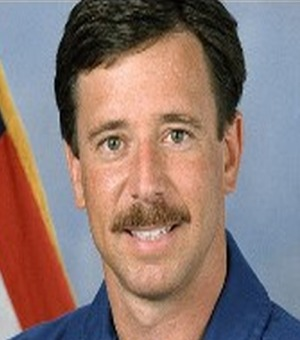
\includegraphics[width=1.55cm]{foto.jpg}};
\node[nota, below=2pt of in] (inl) {una foto};
\node[foto] (mesh) at (2.4, 1.75) {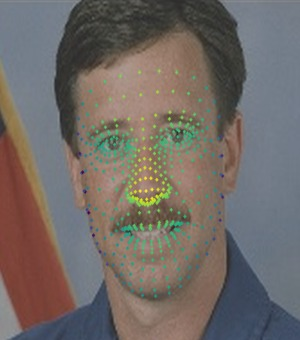
\includegraphics[width=1.55cm]{e_malla3d.jpg}};
\node[nota, below=2pt of mesh] (meshl) {478 puntos con\\profundidad};
\node[paso, text width=3.5cm, minimum height=1.75cm] (build) at (5.75, 1.75) {%
  \textbf{Gaussianas 3D}\\[2pt]
  discos tangentes por área 3D:\\[1pt]
  $\Sigma = R\,\mathrm{diag}(s^2, s^2, (0{,}4s)^2)\,R^\top$\\[1pt]
  más hebras de barba y relieve};
\node[paso, text width=2.6cm, minimum height=1.75cm] (ply) at (9.85, 1.75) {%
  \textbf{Exportar \texttt{.ply}}\\[2pt]
  escala en logaritmo,\\cuaternión, armónico\\de grado 0 y opacidad\\en logit};
\begin{scope}[on background layer]
  \node[grupofondo=muted, fit=(in)(inl)(mesh)(meshl)(build)(ply)] (server) {};
\end{scope}
\node[titulo=muted] at (server.north west) {Servidor $\cdot$ Python};

\node[paso, text width=3.3cm, minimum height=1.6cm] (vertex) at (1.1, -2.05) {%
  \textbf{Vertex shader}\\[2pt]
  $\Sigma_{2D} = J W \Sigma W^\top J^\top + 0{,}3\,I$\\[1pt]
  cuadrilátero de $\pm3\sigma$};
\node[paso, text width=2.55cm, minimum height=1.6cm] (sort) at (4.6, -2.05) {%
  \textbf{Counting sort}\\[2pt]
  65\,536 casillas de\\profundidad, $O(N+K)$};
\node[paso, text width=2.55cm, minimum height=1.6cm] (frag) at (7.75, -2.05) {%
  \textbf{Fragment shader}\\[2pt]
  $\alpha = a\,e^{-r^2/2}$,\\de atrás hacia adelante};
\begin{scope}[on background layer]
  \node[grupofondo=blue, fit=(vertex)(sort)(frag)] (browser) {};
\end{scope}
\node[titulo=blue, anchor=south east] at (browser.north east) {Navegador $\cdot$ WebGL2};

\node[foto] (o1) at (10.55, -2.05) {
\includegraphics[width=1.3cm]{e_frente.jpg}};
\node[foto] (o2) at (11.95, -2.05) {
\includegraphics[width=1.3cm]{e_splats.jpg}};
\node[foto] (o3) at (13.35, -2.05) {
\includegraphics[width=1.3cm]{e_giro.jpg}};
\node[nota, below=1pt of o1] (l1) {de frente};
\node[nota, below=1pt of o2] {cada gaussiana};
\node[nota, below=1pt of o3] {girada};
\node[grupo=green, fit=(o1)(o3)(l1)] (out) {};
\node[titulo=green] at (out.north west) {Resultado};

\draw[flecha] (in) -- (mesh);
\draw[flecha] (mesh) -- (build);
\draw[flecha] (build) -- (ply);
\coordinate (gap) at ($(server.south)!0.5!(browser.north)$);
\draw[flecha] (build.south) |- (gap) -| node[pos=0.25, above=1pt, nota, font=\sffamily\scriptsize\bfseries] {110\,000 a 170\,000 gaussianas} (vertex.north);
\draw[flecha] (vertex) -- (sort);
\draw[flecha] (sort) -- (frag);
\draw[flecha] (browser.east |- frag) -- (out.west |- frag);

\end{tikzpicture}
\end{document}
